\chapter{Xilinx ZCU106}
A feladat megoldására a Xilinx ZCU106 tesztkártyát használtam.\cite{ZCU106}

\begin{figure}[!ht]
    \centering
    \includegraphics[width=150mm, keepaspectratio]{figures/ZCU106.jpg}
    \caption{ZCU106 Tesztkártya}
\end{figure}

\section{Zynq UltraScale+ MPSoC}
A kártya központi egysége egy SoC (System on a Chip). Az SoC két részre osztható.

\begin{figure}[!ht]
    \centering
    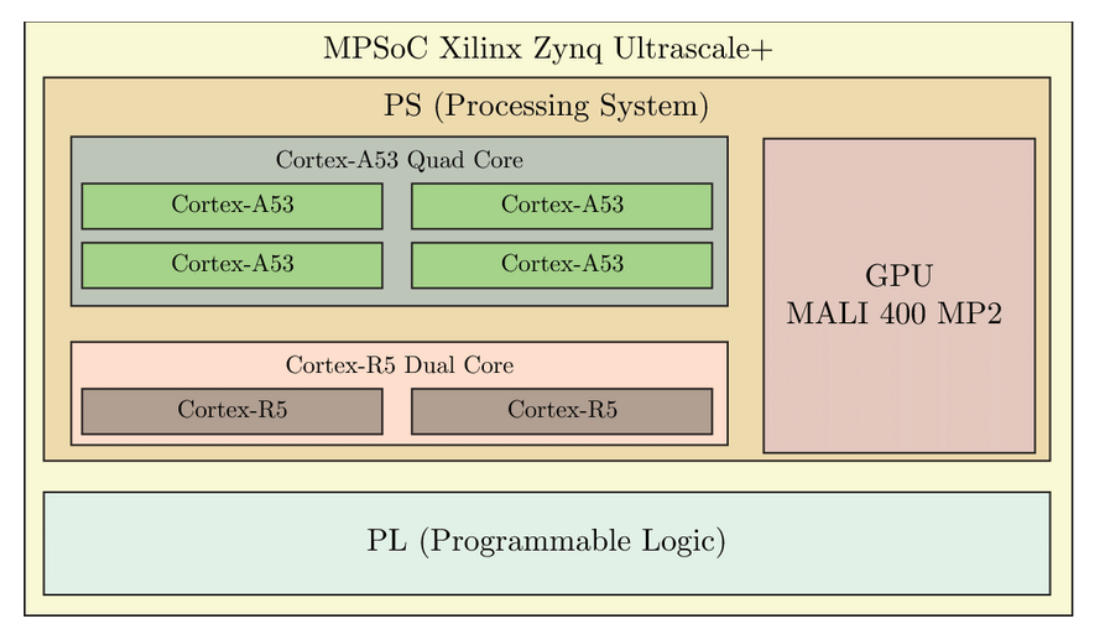
\includegraphics[width=150mm, keepaspectratio]{figures/PS.png}
    \caption{A Processing System blokkvázlata}
\end{figure}

A PL (Programmable Logic) részben, egy FPGA-hoz hasonlóan szabadon lehet hardvert kialakítani valamilyen hardverleíró nyelv segítségével. Ugyanakkor gyakori felhasználása a PL-nak, hogy nem írjuk meg kézzel a hardvert, hanem rendelkezésre álló IP (Intellectual Property) core-okat használunk fel. Az ilyen core-ok általában szoftverrel összhangban, az aktuális program valamilyen lépését képesek hardveresen gyorsítani. Elképzelhető még valamilyen interface, például HDMI interface kialakítása is. Ebben a feladatban leginkább a hardveres gyorsítás van a középpontban.

A PS (Processing System) részben általában leginkább CPU (Central Processing Unit) core-okat találunk. Ebben az SoC-ben található egy négymagos Arm Cortex-A53 processzor, és egy kétmagos Arm Cortex-R5 processzor. Előbbi az általános alkalmazások futtatására alkalmas, míg utóbbi képes valós idejű működésre is. A PS-t lehet használni bare metal alkalmazások futtatására, ebben az esetben a lefordított bináris alkalmazást közvetlenül a CPU-n futtatjuk. Lehetőség van azonban operációs rendszert futtatni a PS-en. Ebben a feladatban is ilyen megoldást választottam. Az operációs rendszer neve Petalinux, és egy későbbi fejezetben kerül majd bemutatásra.

A PS része még egy Arm MALI 400 MP2-es GPU is. A GPU feladata nem a hardveres gyorsítás, erre a célra a PL-ot kell felhasználni. A GPU segítségével lehetőség van videók dekódolására és enkódolására, valamint minimális grafikus megjelenítésre is.

\section{Perifériák és interface-ek}
A ZCU106 kártya számos perifériát tartalmaz, hogy az SoC-t a lehető legtöbb felhasználás esetében lehessen kipróbálni vagy tesztelni. Ezek közül a feladat szempontjából legfontosabbak fogom bemutatni.

\subsection{Memóriák}
A kártya rendelkezik két egységnyi DDR4 RAM memóriával is. Az egyik egy standard SoDIMM memória, amit a PS tud használni csakúgy mint egy normális számítógép. A másik egységen a memória chipek már nem rendelkeznek egy hordozó PCB-vel, hanem közvetlenül a kártyán helyezkednek el. Ezeket a memóriákat a PL-ból tudjuk elérni megfelelő hardver szintetizálásával.

\subsection{Nagysebességű interface-ek}
A kártyán jelen van szinte minden gyakran használt nagysebességű interface. Például rendelkezik egy 4 sávos 4. generációs PCIe csatlakozóval, RJ45 Ethernet csatlakozóval, valamint videó jeleknél használatos portokkal: egy HDMI és egy DisplayPort In/Out csatlakozóval.

A felsoroltak közül a feladat során fel lehet majd használni a DisplayPort csatlakozót, ezen keresztül is tudunk majd videó jelet küldeni az SoC-nak. Ezen kívül használni kell az Ethernet csatlakozót is, mivel a tesztelés során a kártyát távolról kell konfigurálni és az elérés Etherneten keresztül lehetséges.

\subsection{USB csatlakozók}
A kártyán található egy standard USB csatlakozó. A végső megoldás során valószínűleg a DisplayPort-os kamera helyett inkább egy USB interface-szel rendelkező kamera kerül majd felhasználásra.

A kártyán található egy micro-USB csatlakozó amit UART kapcsolat megvalósítására lehet felhasználni. A feladat során ennek is elkerülhetetlen a használata, hiszen ezen keresztül érjük majd el PS-en futó operációs rendszer CLI-ét (Command Line Interface).

\section{IP core-ok}
Az IP core-ok kicsit kilógnak a sorból, hiszen nincsenek rajta fizikailag a kártyán, viszont valamilyen módon mégis kapcsolódnak hozzá. Az IP core-okat a Xilinx szolgáltatja a tesztkártyákhoz, és ezek használata sokszor függ attól, hogy milyen módon vagy célra vásároltunk, és hogy milyen tesztkártyát.

A feladatban két lényeges IP core-t kell felhasználni. Az egyik a DPU (Deep Processing Unit), amit már az eddig elkészült tesztek során is fel tudtam használni. Ennek feladata, ahogy az a nevéből is látszódik, a mély neurális hálózatok, pontosabban ezek kiértékelésének hardveres gyorsítása.

A másik IP core felhasználása a tárgy második felében fog megvalósulni, ez a Multiscaler IP core lesz. Ennek feladata képek átméretezése.
